\section{Materials and Methods}
\label{sec:matmet}

In this section, we present the materials used in the research - the British spatial
signatures we would like to identify and Sentinel 2 satellite
imagery - and methods designed to understand our ability to train a conventional model on
such a task and to unpack the role of geography in image-based deep learning.

\subsection{Materials}

The research uses only two data inputs, one representing the "ground truth" we aim to
predict using neural networks and the other representing satellite
imagery. While the latter does not need much introduction, the British spatial
signatures used as labels need to be explained further.

\subsubsection{British Spatial Signatures}
% 500 words

Spatial signatures are a classification of space covering the entirety of a case
study area. They are defined as \textit{"a characterisation of space based on form and
function designed to understand urban environments"} \citep{dab_mf_2021a}. This
definition points at the clear distinction between signatures and traditional
LULC classifications. Taking the example of CORINE
\citep{europeanenvironmentagency1990} as a representative of LULC, it has 44 distinct
classes, out of which 2 cover urban form, and six other can be loosely related to urban
areas\footnote{Continuous urban fabric, Discontinuous urban fabric; Construction sites,
Green urban areas, Sport and leisure facilities, Industrial or commercial units, Road
and rail networks and associated land, Port areas}. A similar situation arises with recently
released global LULC datasets. European Space Agency's WorldCover project distinguishes
11 classes, of which one is urban (Built-up) \citep{zanaga_daniele_2021_5571936}. Esri's
Land cover has 9 classes: one is \textit{Built Area}, and the rest covers unbuilt
areas \citep{karra2021global}. This ratio of built vs unbuilt classes is typical but not
very suited for research applications focusing on urban environments. Spatial signatures
invert this ratio as they are primarily classifying urban space.

There are two main concepts embedded in spatial signatures delivering urban-focused
classification. The first one is the spatial unit called the enclosed tessellation cell
(ETC). To derive ETCs, \cite{dab_mf_2021a} first generate \textit{enclosures}, spaces fully enclosed by
a set of barriers (roads, railways, rivers, coastline). ETCs are an outcome of
Voronoi tessellation based on building footprint polygons. The resulting spatial unit
has adaptive granularity reflecting the scale of each urban pattern. The
second is the selection of characters describing each ETC. They measure form and function,
primarily urban phenomena and mostly omit environmental aspects focusing on land
cover patterns. However, spatial signatures depend on a wide range of data inputs that
are being updated at a variable rate. Some in monthly snapshots but others,
based on census data, only every ten years. Given this heterogeneity,
it is nearly impossible to provide a consistent yearly time series of their evolution.
This is where remote sensing based on satellite imagery may help.

% We may want to add a figure explaining ETCs here.

As presented in \cite{fleischmann2022geographical}, British spatial signatures are one
application of the concept of spatial signatures in
the context of Great Britain. It divides the space into 16 data-driven classes
(Figure \ref{fig:signatures}) listed in Table \ref{tab:sig_types}. Out of these 16
classes, nine are entirely urban, four are peripheral, and only three classify natural spaces,
inverting the ratio of built vs unbuilt classes common in LULC. However, out
of these 16 classes, some are very rare, and it would not be feasible to attempt to
predict them. Therefore, we merge five classes under the "urbanity" group into a
single one and use the resulting 12 classes throughout this paper, while using entirety
of Great Britain as a study area.


\begin{table}
\begin{tabular}{lrrrr}
    \toprule
    {} &        area (sq.km) &  ETC count &  area (\%) &
    ETCs (\%) \\
    Signature type                       &             &         &            &
    \\
    \midrule
    Countryside agriculture              & 93,856.1 & 3,022,385 &         41 &
    21 \\
    Accessible suburbia                  &  2,244.5 & 1,962,830 &          1 &
    14 \\
    Dense residential neighbourhoods     &    957.2 &   502,835 &          0 &
    3 \\
    Connected residential neighbourhoods &    565.4 &   374,090 &          0 &
    3 \\
    Dense urban neighbourhoods           &    570.6 &   238,639 &          0 &
    2 \\
    Open sprawl                          &  5,081.5 & 2,561,211 &          2 &
    18 \\
    Wild countryside                     & 91,306.3 &   595,902 &         40 &
    4 \\
    Warehouse/Park land                  &  2,462.4 &   707,211 &          1 &
    5 \\
    Gridded residential quarters         &    261.2 &   209,959 &          0 &
    1 \\
    Urban buffer                         & 31,588.8 & 3,686,554 &         14 &
    25 \\
    Disconnected suburbia                &    708.9 &   564,318 &          0 &
    4 \\
    Local urbanity*                       &    231.1 &    86,380 &          0 &
    1 \\
    Concentrated urbanity*                &      7.8 &     1,390 &          0 &
    0 \\
    Regional urbanity*                    &     76.4 &    21,760 &          0 &
    0 \\
    Metropolitan urbanity*                &     16.5 &     3,739 &          0 &
    0 \\
    Hyper concentrated urbanity*          &      2.2 &       264 &          0 &
    0 \\
    \bottomrule
\end{tabular}
    \caption{\label{tab:sig_types}Classes of British spatial signatures and their
    coverage in terms of area and a number of ETCs. Urbanity classes marked with * are
    combined for the experiments presented in this paper.}
\end{table}


\begin{figure}
    \centering
    \begin{subfigure}[b]{0.8\textwidth}
        \centering
        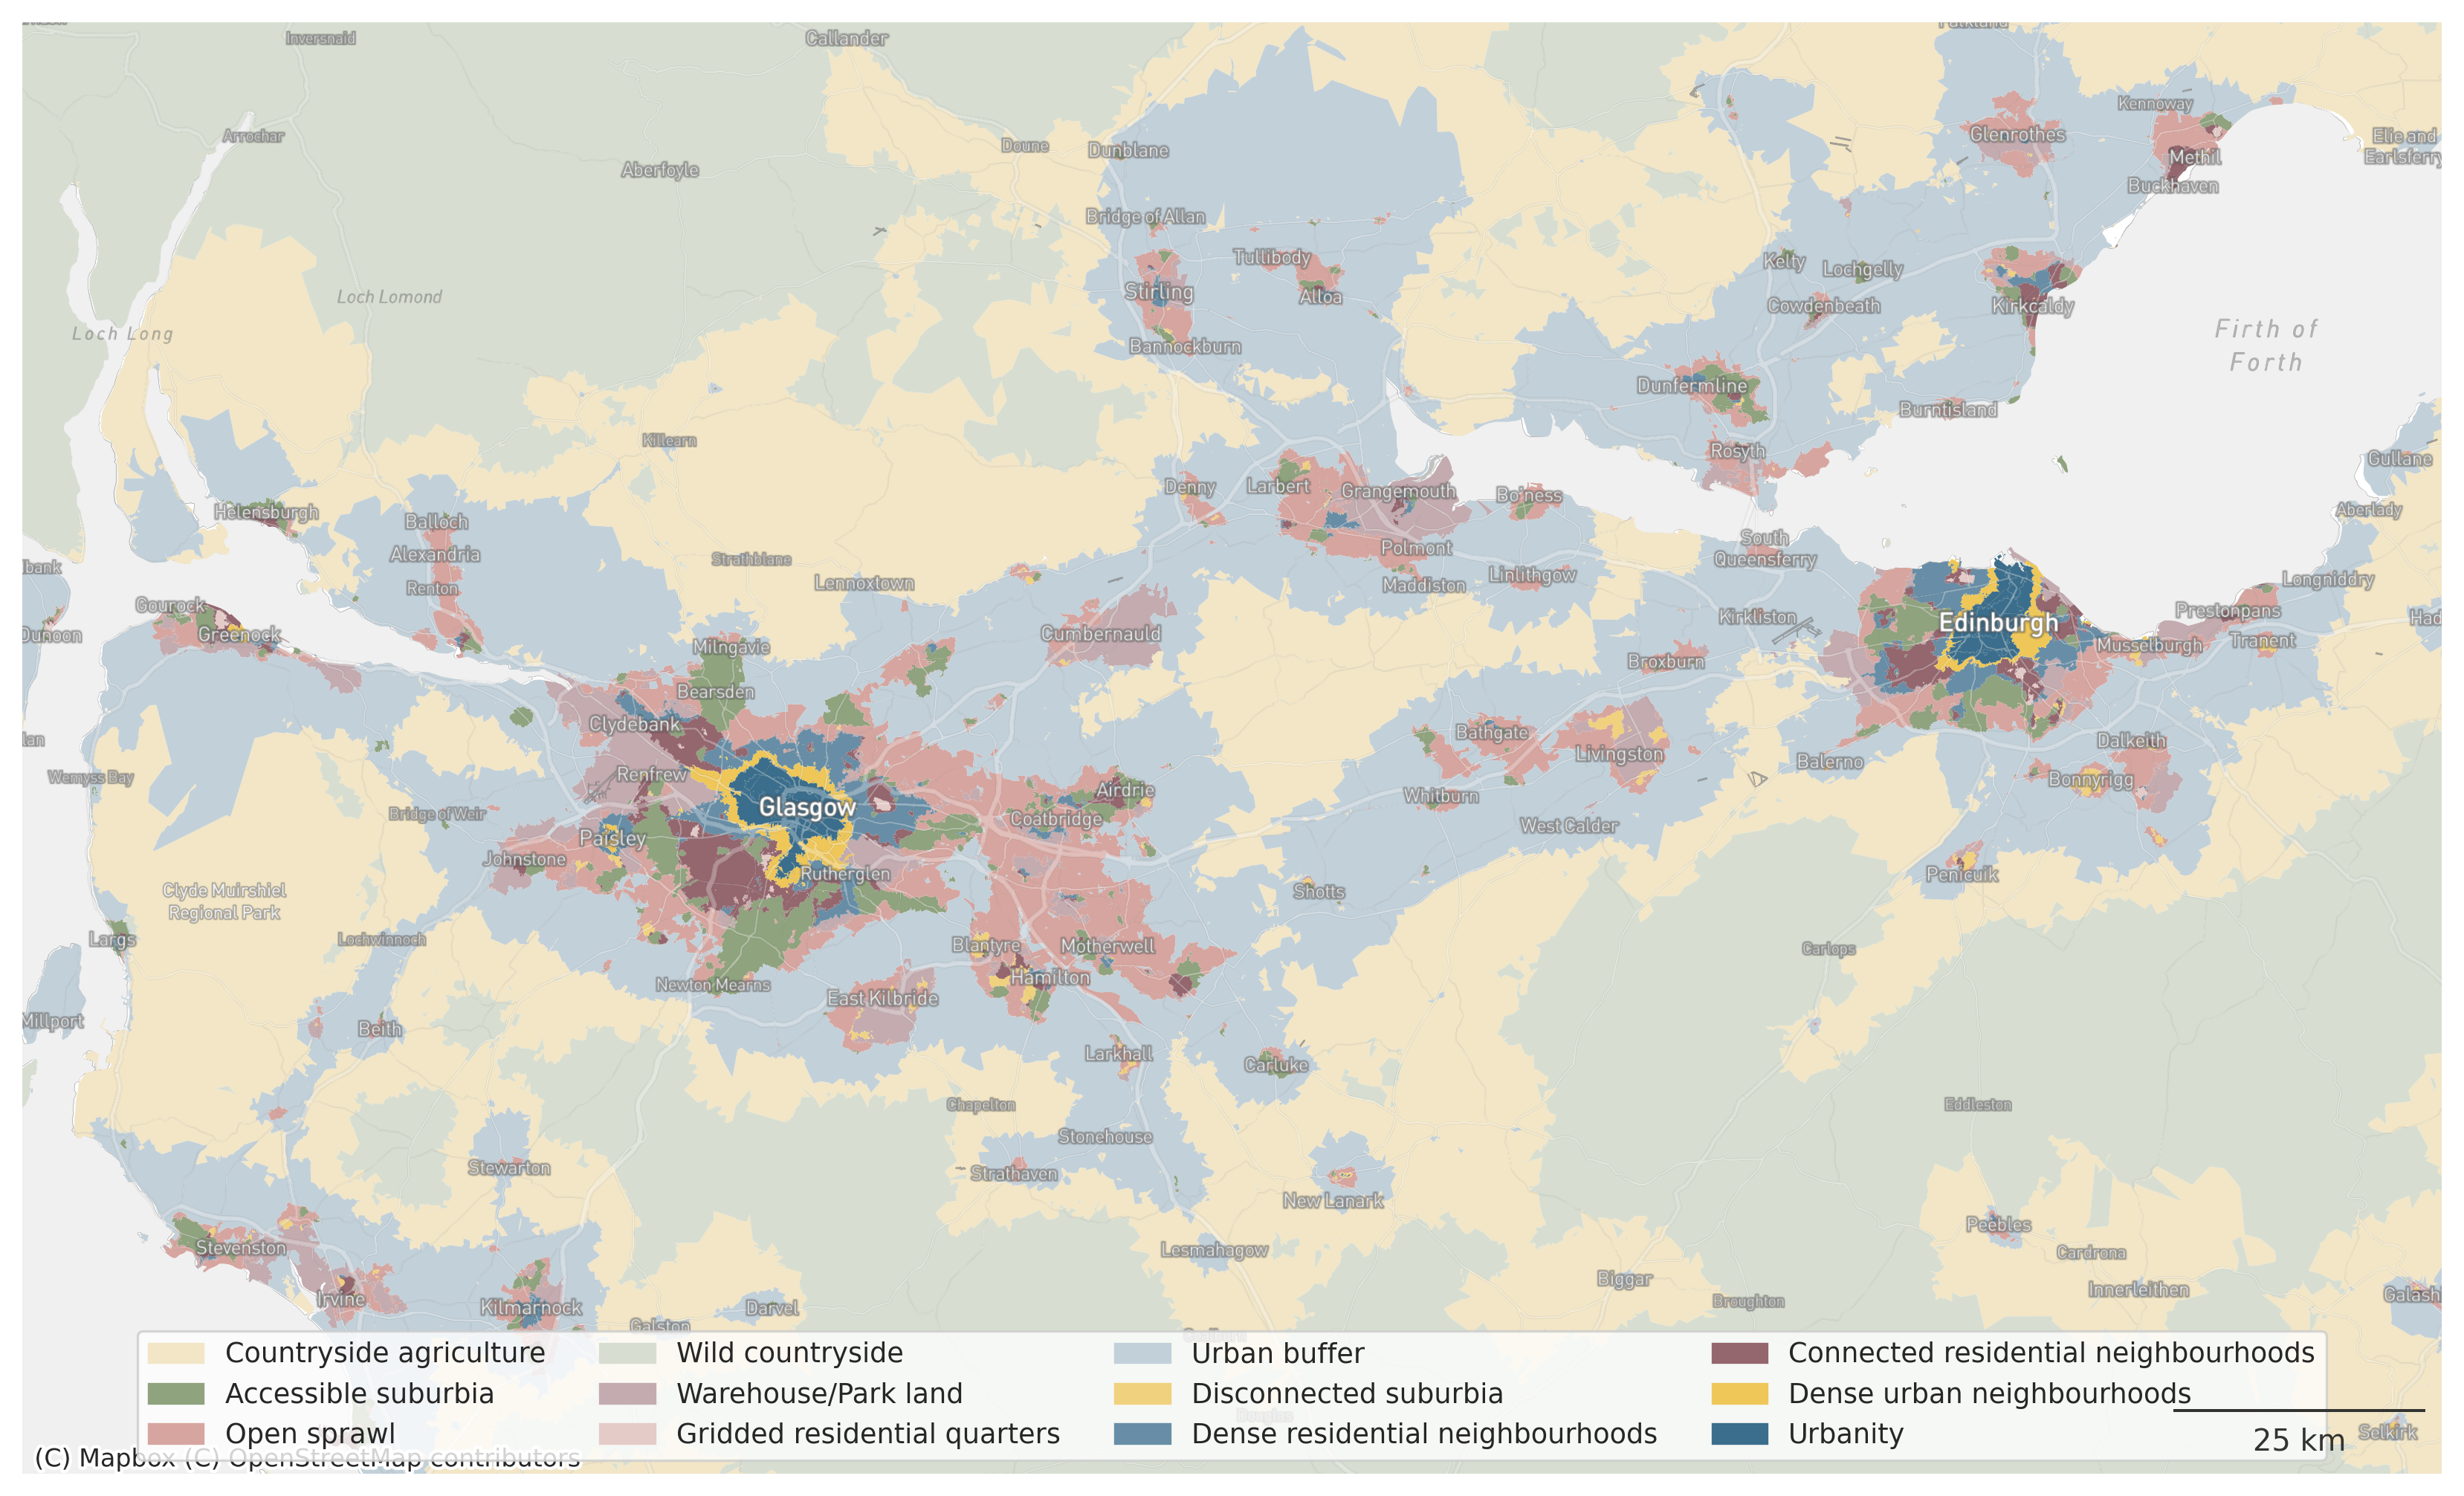
\includegraphics[height=8cm]{fig/signatures_scottish_belt_12_classes.png}
     \end{subfigure}
    \hfill
    \begin{subfigure}[b]{0.19\textwidth}
        \centering
        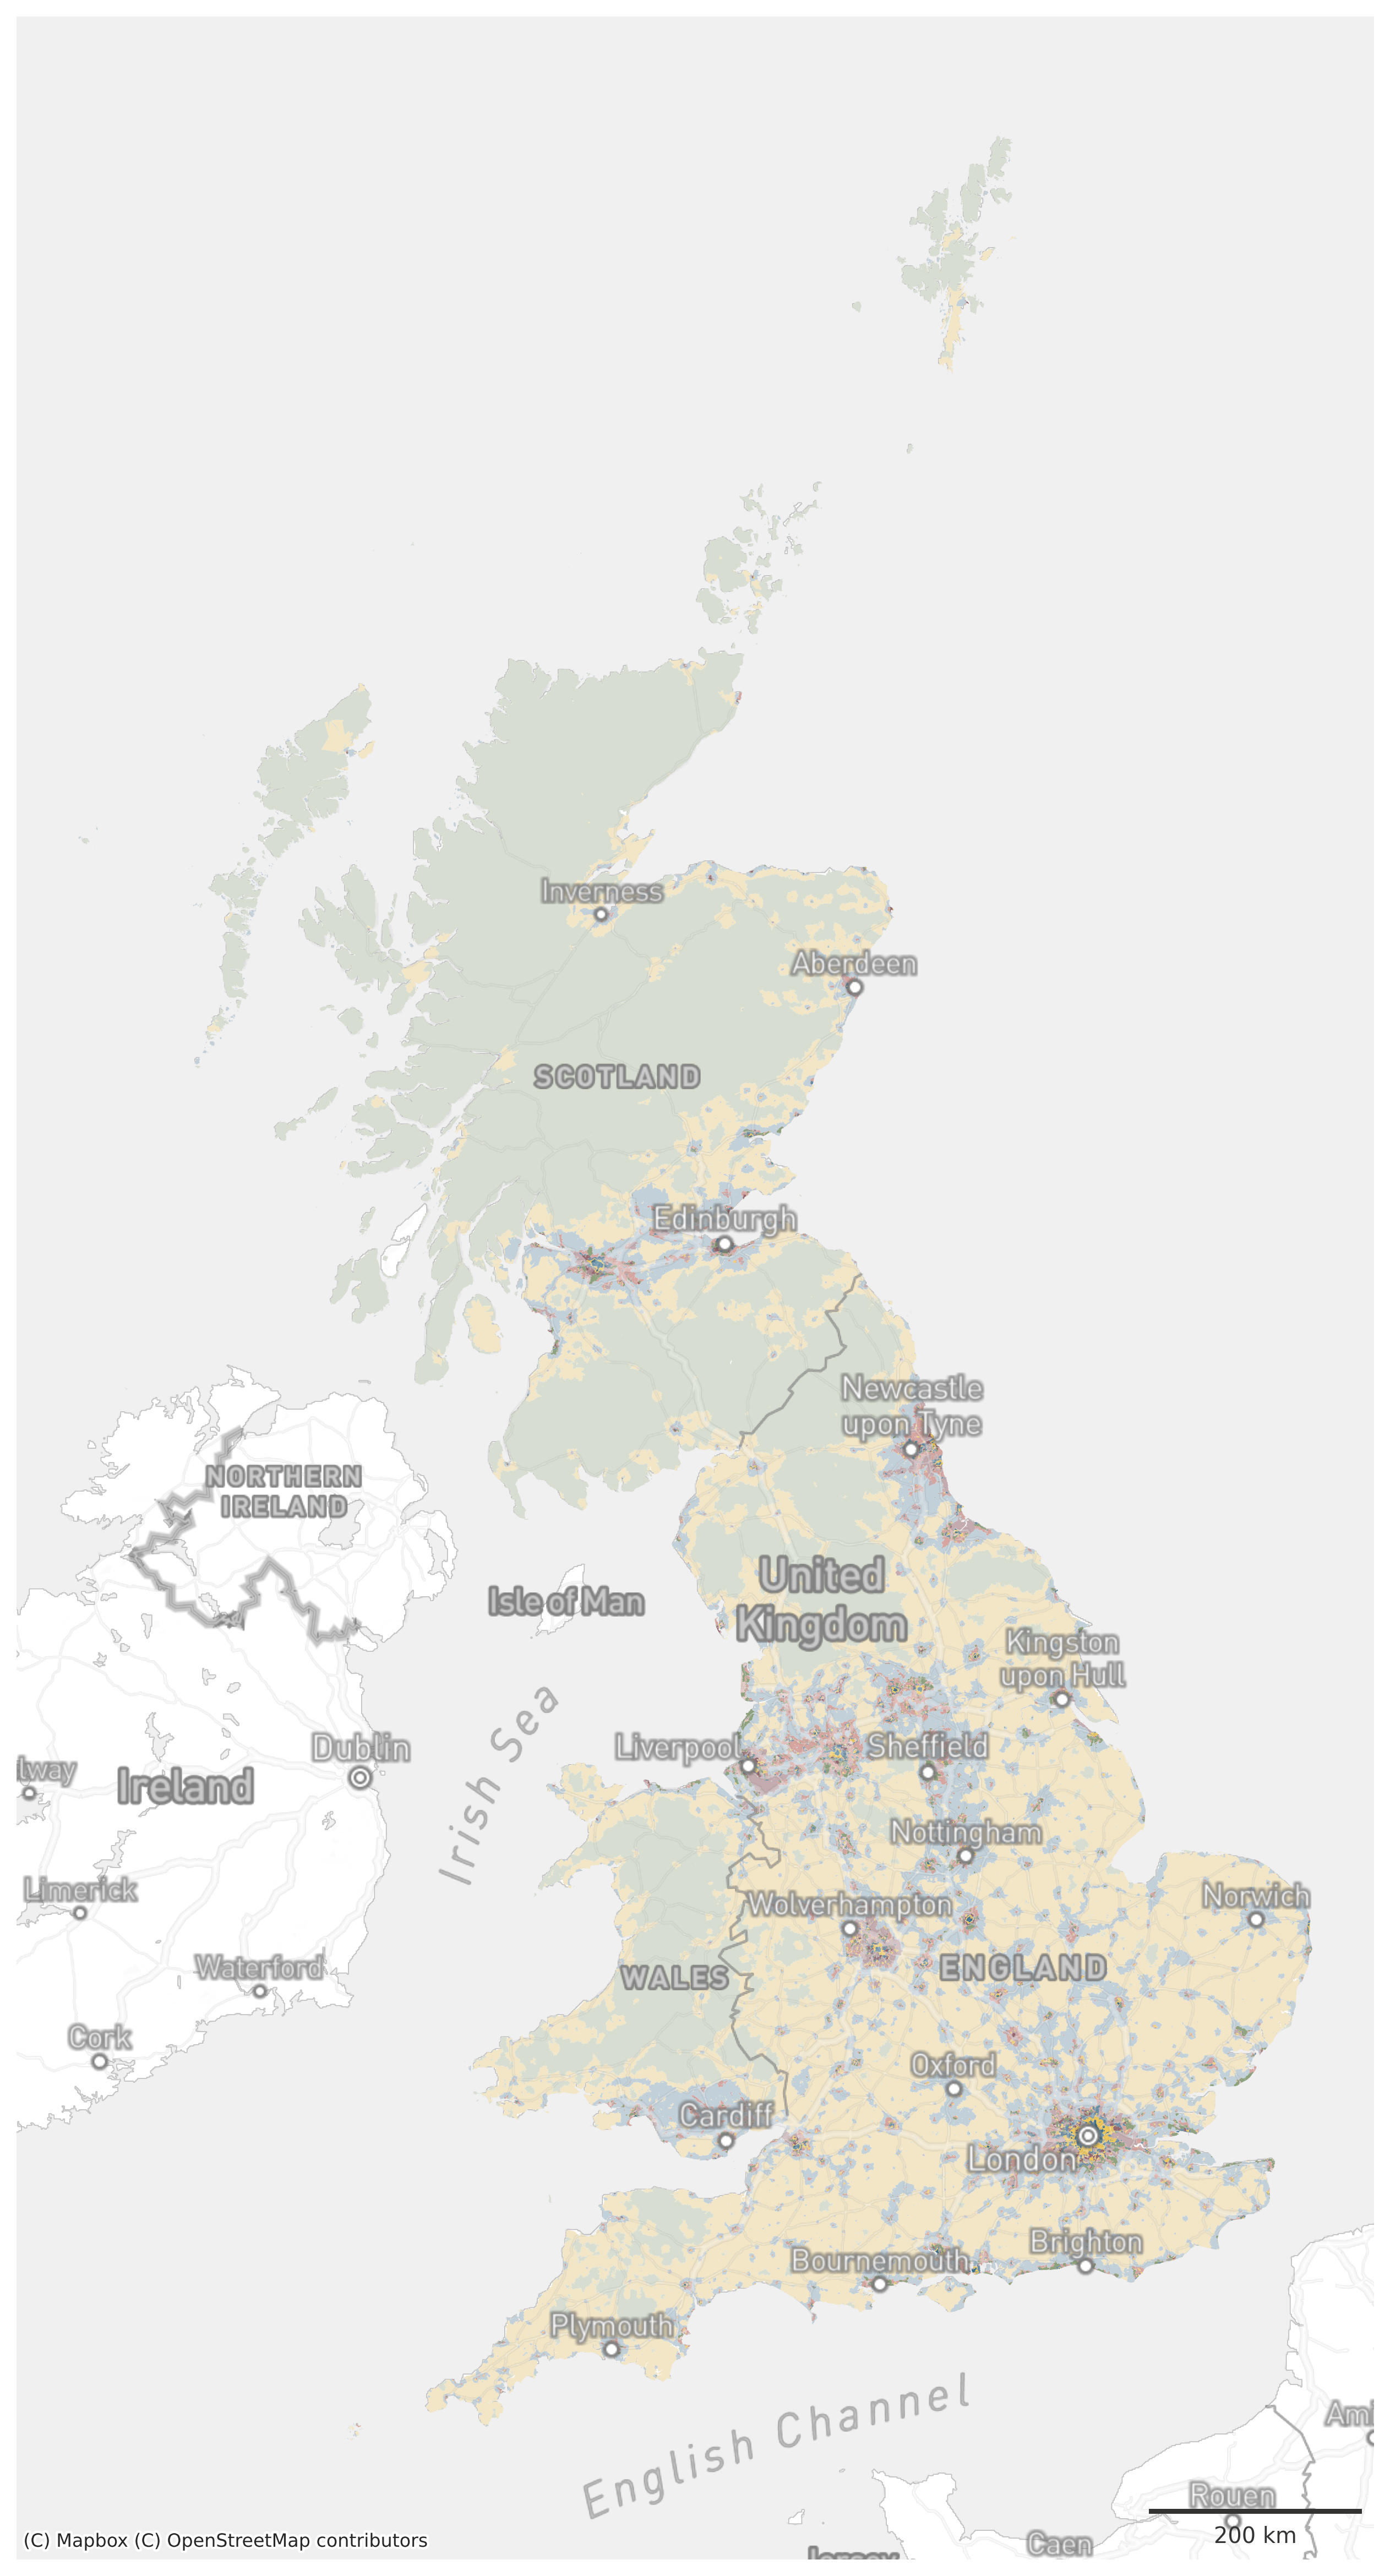
\includegraphics[height=8cm]{fig/signatures_gb_12_classes.png}
    \end{subfigure}
\caption{Spatial signatures in the full extent of Great Britain and zoomed to a
metropolitan area of the Scottish Central Belt stretching from Glasgow to Edinburgh,
limited to 12 classes used in this paper.}
\label{fig:signatures}
\end{figure}


\subsubsection{Sentinel 2 imagery}

% 250 words

The second data input used in this research is satellite imagery provided by the
Sentinel 2 mission. Specifically, we use the pre-processed cloud-free mosaic of Sentinel
2 released by \cite{CORBANE2020105737}.
The mosaic provides pixel-level composite based on imagery for the period January 2017-
December 2018 at an original resolution of 10 meters per pixel. While Sentinel 2
captures many spectral bands beyond traditional visible red, green and blue (RGB), this
research uses only RGB bands due to its employment of pre-trained neural networks
stemming from non-satellite imagery that is composed only of RGB and an attempt to
minimize training from scratch that would need to happen to derive weights for other bands. The exclusion of other
bands may be seen as a limiting factor of the work, but we believe that, as with other
aspects that will be discussed later, it efficiently illustrates the \textit{lower
bound} of the performance of the presented method and can be only improved with the addition of
other spectral bands or other data (e.g. synthetic-aperture radar imagery).

Another notable aspect of the Sentinel 2 imagery is the resolution. Ten meters per pixel
may be enough to distinguish LULC classes, as shown by the examples discussed
above. However, it is unclear whether it is enough to delineate types of urban
environments. Individual buildings often do not stretch beyond the spatial extent of two
pixels, which is severely limiting what we can \textit{see} on the image, as illustrated
in Figure \ref{fig:chips}. While other data sources may provide better
resolution\footnote{For example, commercial imagery by Maxar reaches a resolution of
30cm per pixel and imagery by Planet of 50cm per pixel}, potentially improving model
performance, this research is bound within the limits of \textit{open data}, where
Sentinel 2 is the best offering to date.


\subsection{Methods}

% 250 to explain the overarching experiments

We define our challenge as an image classification task and use competing alternatives
to explore which one performs best and to assess whether the \textit{best} is good enough.
Each of them implies geographically relevant
trade-offs. First, we build and train a model composed of a convolutional neural network
and probability modelling able to predict the 12 classes derived from the spatial
signatures. Second, we use methods designed to unveil which of the inherently
geographical decisions being tested has a significant effect on the resulting
performance and should therefore be considered when applying CNN to spatial
problems.

When selecting the CNN architecture, we have intentionally excluded image
segmentation. While it seems like an ideal candidate for the task at hand, there are
several reasons for its exclusion. The first has to do with the spatial signatures and the
nature of the boundaries between individual types. While the dataset from
\cite{fleischmann2022geographical} delineates them with hard boundaries when one cell
is a type A and the neighbouring one a type B, the reality is not that simple, and these
boundaries should be treated more as a fuzzy edge that the hard one. There is very rarely an immediate
switch between one type of urban environment and the other one. In many cities, two
types tend to form a transition on the edges where neither is dominant. A situation like
this is very challenging for the image segmentation as it often looks at delineation of
water bodies, buildings or other precisely defined patches on an image. The second reason is that the image
segmentation, having a prediction for individual pixels, would not allow us to use the
second part of the method and test the effect of spatial lag in modelling efficiently. The only
way of doing that would be to run the experiment on a pixel level which would be
extremely computationally expensive, hence challenging to reproduce. We believe that the
method that can be run on a local machine is in the end, more valuable than the one
requiring a high-performance cluster.

Overall, our exercise is structured as a comparison of models that attempt to
predict the 12 spatial signatures entirely from Sentinel 2 imagery. Each model 1) takes
a set of training data as input; 2) runs the class prediction using the convolutional neural
network (CNN); and 3) builds a (spatial) model on top of the resulting probabilities. The
differences between the models are capturing the geographical options that are being tested:
extent of the area sampled from the satellite imagery into a single \textit{chip},
presence of spatial augmentation, class exclusivity within each chip, and an
architecture of probability modelling on top of a prediction coming from the CNN.
Finally, the performance of each model is assessed using both traditional non-spatial
techniques used in deep learning and bespoke spatial metrics. Given a large number of
resulting values, a regression approach is used to determine the effect of the tested
options.
Each of the steps is further discussed in detail in the subsequent sections.

\subsubsection{Chip size}

% 500 words

The first question that needs to be answered when trying to apply a classification
algorithm on satellite imagery that spans a large amount of continuous land is how
to sample such data into individual patches (or, hereafter, chips)
that can be assigned to classes. Pre-trained CNNs usually expect a square image of
a certain size, but that does not mean that the same size (in terms of pixels) needs to
be directly sampled from the image, thanks to possible resampling. What should be
retained, though, is the ratio. Therefore, we need to sample square chips of a
custom size. Within an image classification framework, which is the first type of model that is tested, we assume that
each chip contains data of a single class only. Therefore, such a chip should be entirely
within the boundary of a single signature type. That poses some restrictions as spatial
signatures, especially in the urban context, tend to be relatively granular, and large chips
would not fit inside the boundaries, reducing the number of
valid chips for training. Therefore, the goal is to find a balance
between the number of chips sampled from the data and the amount of
information each chip can hold. Given the relatively coarse resolution of Sentinel 2, a
chip of 100x100 meters consists of only 10x10 pixels, which may not be enough to capture
the nature of a signature type and distinguish it from other types. On the other hand, a
chip of 1000x1000 meters, which is likely large enough to capture the difference, will
not fit in most of the signature boundaries and we would end up with only a few chips per
urban class.

The literature rarely discusses the decisions involved in defining the chip
size for single-class chip classification. In some cases, the size is predetermined due to the requirement of either a
pre-trained model or an existing set of labelled data \citep{taubenbock2020}. In
others, the size that has
been used in previous studies is applied again without discussing the implications
of such a decision \citep{wang2018mapping}. From a spatial analysis
perspective, this approach is surprising as deciding the chip size is a prime example of the
modifiable areal unit problem (also known as MAUP,
\citealp{openshaw1981modifiable}), especially the aspect about scale, which states that
a change of the scale may affect the outcome of an experiment. Hence such an effect
should be at least considered in an interpretation if not minimized where possible.

In this work, we try to understand the effect of chip size by testing all the models
based on four different chip sizes - 80, 160, 320 and 640 meters representing chips of
8x8, 16x16, 32x32 and 64x64 pixels, respectively, illustrated on a Figure \ref{fig:chips}
and a Supplementary Figure \ref{fig:chip_fits}.


\begin{figure}
    \centering
    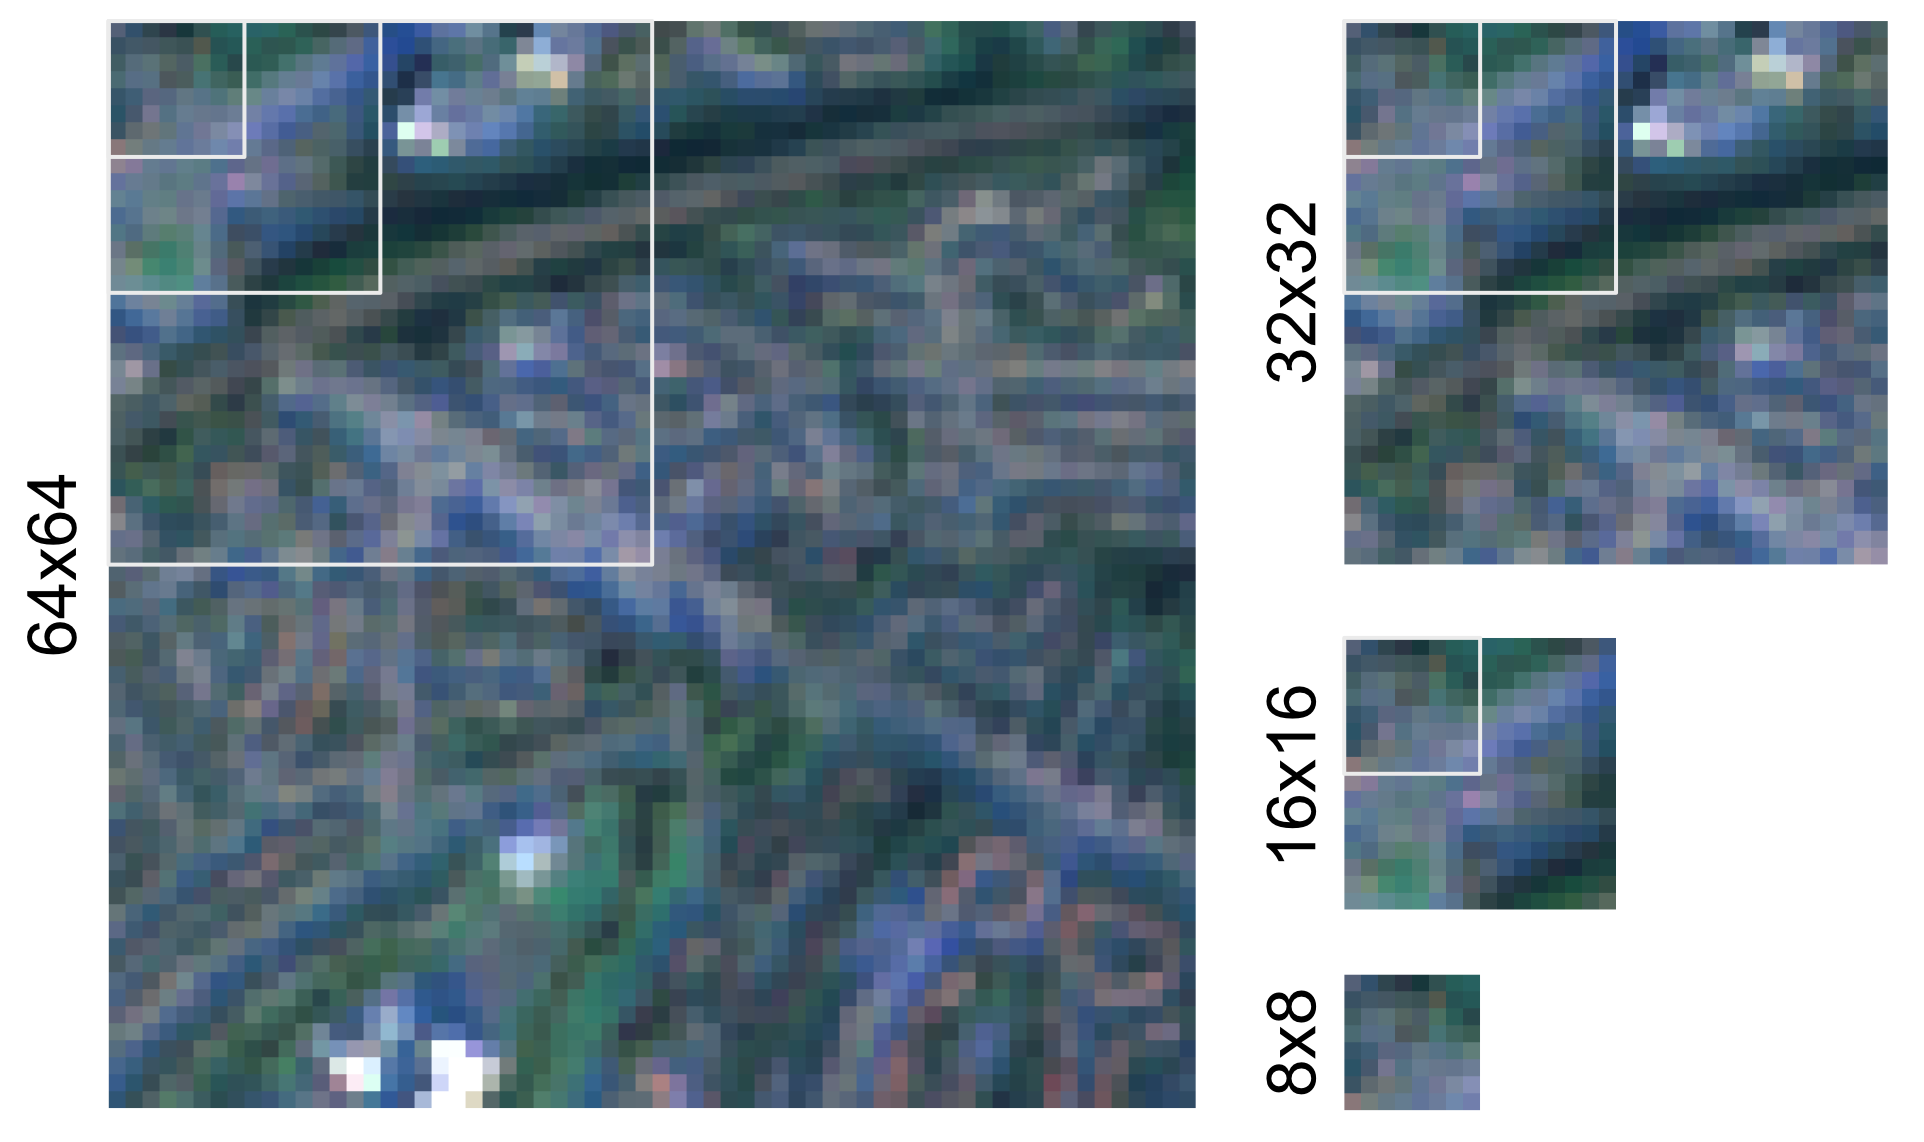
\includegraphics[width=.8\linewidth]{fig/chips.png}
    \caption{Illustration of the selected chip sizes using the Sentinel 2 cloud-free mosaic. Each of the chips also shows the sizes of the smaller options as a white outline.}
    \label{fig:chips}
\end{figure}



\subsubsection{(Spatial) data augmentation - \textit{Sliding}}

% Sliding

% 250 words

As mentioned above, in combination with the signature geometry and
the requirement to keep chips exclusively within a single class, specific chip sizes may result in
insufficient training data for some signature types causing imbalance in the training set. Under-sampling like this
one can be a serious problem that is not unique to spatial modelling. However,
traditional augmentation methods are not directly applicable here. For example, in an
image classification problem trying to determine if there is a cat or a dog on an image,
we add some rotation or zoom to get more versions of
the same image and expand the set of training data. Neither of these methods is
applicable to spatial problems. Rotating the image would break
natural light conditions, while zooming in would change the scale of the urban environment
we attempt to capture. Moreover, distinction between some signature types is partially
in different orientation of streets, rendering rotation-based augmentation counter-productive.

At the same time, the geographical and continuous nature of the data at hand
allows us to use explicitly spatial augmentation techniques such as the one we
call \textit{sliding}.
Sliding can be seen as overlapping sampling. Instead of overlaying a grid of chips over
target geometry and using each pixel only once, we take the initial grid and slide it a
few pixels horizontally and vertically, as illustrated in Figure \ref{fig:sliding}. If
the boundary of a slid chip is fully within a signature geometry, it is added to the
pool of chips to be used. This process is done repeatedly to ensure that each class has
a reasonable amount of chips to work with, while chips from the large signature types
are intentionally undersampled to retain a relative balance between the classes in the training data.

It is to be noted that sliding can cause data leakage (sequences of pixels being
present in both training and validation) if done before splitting the data into
training and validation subsets. Therefore, we first create the initial grid, subdivide
it spatially into four parts (40\% for CNN training, 10\% for CNN validation, 40\% for
probability modelling training, 10\% for probability modelling validation) and apply
sliding within each part to avoid any pixels being shared among chips from different
sets. Subdivision into the four parts is done within each signature geometry to avoid
potential geographical bias.

\begin{figure}
    \centering
    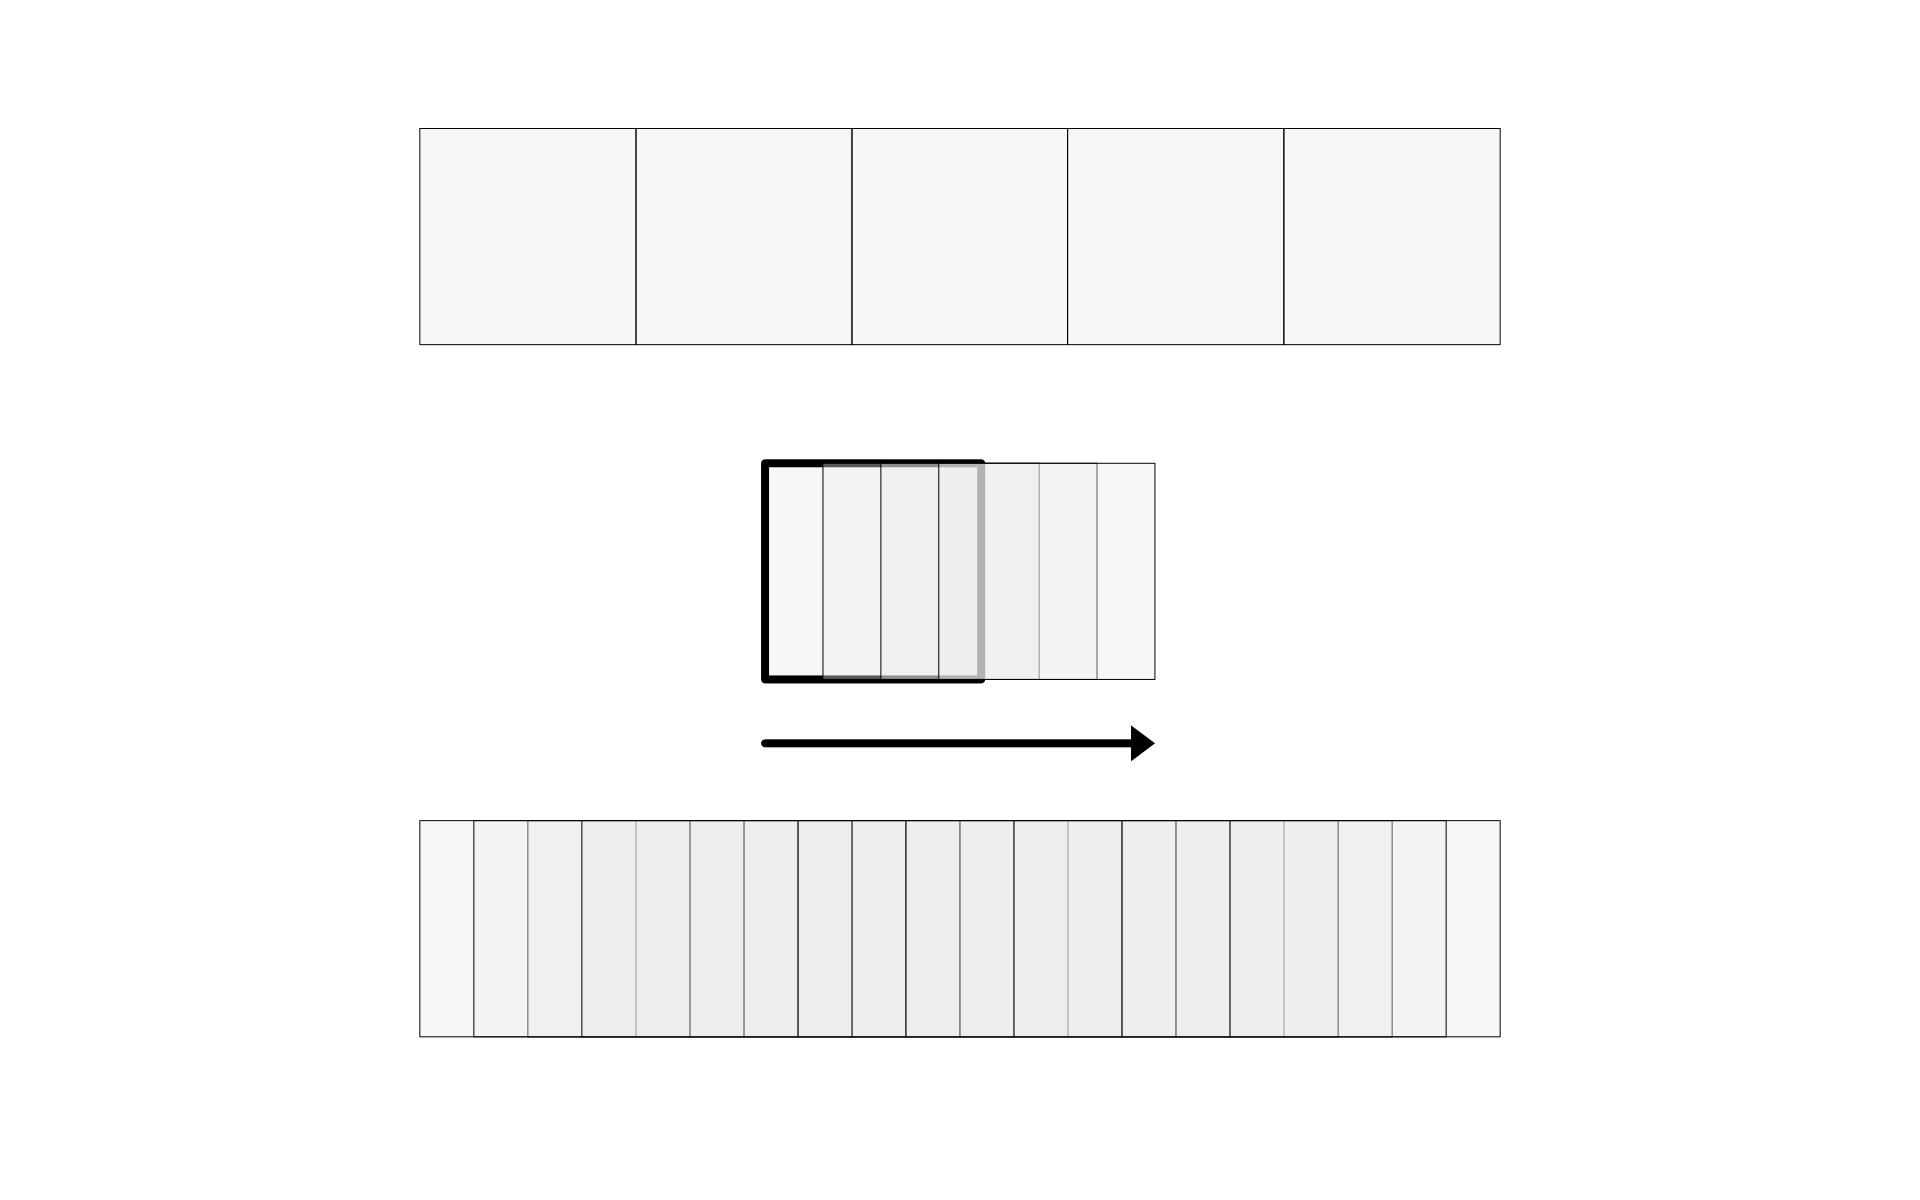
\includegraphics[width=.8\linewidth]{fig/sliding.png}
    \caption{Diagram illustrating the sliding mechanism. The first row shows the initial non-overlapping grid, the last one final overlapping set of chips.}
    \label{fig:sliding}
\end{figure}


\subsubsection{Model architecture}

% 500 words

% Overall content of the section

Model architecture refers to the analytical pipeline that transforms chips
into a prediction for a single signature type. Our competing architectures
contain two main parts. First is a CNN that transforms a single chip into a
set of 12 probabilities, one for each signature type.
Second is a mathematical function that converts such probabilities (
considering only those for the chip of interest or in conjunction with
those of neighbouring chips) into a
prediction for a single signature type. This section describes each of these in detail.
We would like to highlight that, contrary to the majority of deep
learning-focused research, our focus is not on the architecture of the CNN
itself. We assume the effect of geographic choices will largely show similar
behaviour irrespective of the network architecture. For that reason, throughout
our experiments we use \texttt{EfficientNetB4} \citep{https://doi.org/10.48550/arxiv.1905.11946}, pre-trained
on the popular ImageNet dataset \citep{deng2009imagenet}. Appendix \ref*{sec:appendixA} shows a brief comparison of
several standard neural network architectures and their performance on a subset of data
to motivate our decision. We then apply transfer learning by re-training the
top layer of the pre-trained model and replacing it by a
custom sequence of dense layers described below.

% Standard image classification
We consider three variants of the CNN.
The default approach (which we will refer to \texttt{bic}, for ``baseline
image classification'') is a standard image classification problem, using the sets of chips
that are fully within a single signature type. The custom top layer of the pre-trained CNN then contains a Global Average
Pooling (2D) layer, a dense layer with ReLu activation and 256 neurons, and a dense
layer with the softmax activation and a number of neurons equal to a number of classes
(12). The result for a single chip is a collection of 12 probabilities
of a chip belonging to each signature type. The sum of all probabilities is
one.
An extension of this approach (\texttt{sic}, for ``sliding image
classification'') applies this technique to the data being spatially augmented
with the sliding technique described above.

% Multi-output regression
Our third approach recasts the image classification task as a multiclass
prediction. If we relax the requirement that every chip is fully within
the boundaries of a single signature type, we end up with many more available
chips, but now some of them include more than a single label within their
extent. Instead of a single label per chip, we now deal with a 1-D array of them.
This can be beneficial from the geographical perspective as such chips now inherently
encode the co-location of individual signature types and a model could use this information
during the prediction. As signature types usually tend to neighbour only a subset of
other classes (e.g., Urbanity never neighbours Wild Countryside), we can assume that
information on co-location can positively impact predictive performance. We
then include a set of chips sampled from a grid crossing the boundaries of
signature types (using the same chip sizes as before) and adapt the CNN to
perform multi-output regression (\texttt{mor}) instead of image classification. This change
implies the top layer is now composed of a Global Average Pooling (2D) layer, a
dense layer with ReLu
activation and 256 neurons, and a dense layer with the sigmoid activation and a number of
neurons equal to a number of classes (i.e., 12). The result for a single chip is a similar
collection of probabilities, but these are now predicted proportions. As such,
the sum of all of them ranges between 0 and 12 rather than between 0 and 1.

A comparison of the total
number of chips used by each CNN is available in the supplementary table \ref{tab:chip_counts}.
The split of chips is then 40\% for CNN training, 10\% for CNN validation, 40\% for
probability modelling training, 10\% for probability modelling validation equally across all the options.
All CNN models are trained using the following hyperparameters: number of
epochs: 200, optimizer: Adam, patience: 5, and a batch size: 32. See the relevant code
in the linked repository for details.

% Spatial modelling of probabilities TODO: Dani, from this section below are your bits.
The second step in the pipeline takes chip probabilities and turns them into
predictions of a signature type. To do this, we compare five approaches of
differing complexity and sophistication. These five variants stem from the
combination of two components: the set of inputs used to make the prediction and
the function transforming them into a single signature type. For a given chip
$i$, we can express this step of the pipeline mathematically as follows:

\begin{equation}
\begin{split}
        S_i & = f(P) \\
        P & = \underbrace{
                \sum_{k} P_{k-i}
        }_\text{baseline}\;
        \underbrace{
        \left[+ \sum_{k} \sum_j w_{ij} P_{k-j}\right]
}_\text{wx}
        \label{eq:sp_model}
\end{split}
\end{equation}

where $S_i$ is the prediction for the signature type of chip $i$ (one of the $k$ available, where
$k=12$ in our case) and $f(\cdot)$ is a function that
transforms the inputs $P$ into $S_i$. The five
approaches we compare derive from the different implementations of $f(\cdot)$
and $P$. On the latter, we compare models that only use the probabilities
$P_{k-i}$ generated by the CNN for chip $i$ (\texttt{baseline}) with alternatives
(signalled with the \texttt{wx} term) that, in addition,
also include an average of $P_{k-j}$ probabilities, which are the
probabilities generated by the CNN for each neighbour $j$ of chip $i$. This is
akin to what in spatial analysis is called the \textit{spatial lag} of each
probability, and is calculated using a spatial weights matrix $W$ that records
the spatial relationship between every chip in the set. In our $W$, two
neighboring locations $i$ and $j$ will receive a weight $w_{ij}=1$,
if they are in the same of the four split sets as defined above, and if they
either are geographically contiguous or are nearest neighbours; while otherwise
they will be considered non-neighbours and receive a weight $w_{ij}=0$. To obtain
an average of the neighbors, we row-standardise $W$ so that $\sum_j w_{ij} =
1$. The second dimension other than $P$ we vary is the function $f(\cdot)$ that converts
it to the prediction $S_i$. We take three distinct approaches here: simply
picking the maximum probability (\texttt{maxprob}), which we only use without the spatial lag of
probabilities; an ensemble of binary logit models to predict each class
(\texttt{logite}), then selecting the class with top probability, which we
also use with the \texttt{wx} variant; and a histogram-based gradient boosted
classifiers inspired by LightGMB \citep{ke2017lightgbm} and implemented in
\texttt{scikit-learn} \citep{pedregosa2011scikit}. This yields our five
competing models:
\texttt{maxprob}, \texttt{logite\_baseline}, \texttt{logite\_baseline-wx},
\texttt{HGBC\_baseline}, and \texttt{HGBC\_baseline-wx}.

\subsubsection{Performance metrics}

% 500 words
The goal of our experiments is to compare different models under varying
geographical conditions to learn both which performs best, but also how
different choices of geographical nature influence the overall performance
when predicting form and function from satellite imagery.
To provide a workbench that systematically compares each model and setup, we
use a set of performance scores that operate either at the global or class level,
and that measure performance in the traditional machine learning sense, as
well as in the spatial sense.

% Traditional non-spatial
We use four standard performance scores. \textit{Cohen's kappa} score ($\kappa$,
\citealp{cohen1960coefficient}) is a measure of agreement between two sets of
categorical labels that ranges from -1 to 1. Intuitively, it measures the
extent to which the two sets agree with each other (i.e., same label for the
same observation) beyond what would be expected from pure chance
($\kappa=0$). Cases where there is more disagreement than expected from chance
receive a negative score. \textit{Global (within-class) accuracy} captures the
proportion of observations correctly predicted (in a given class). The
\textit{Macro F1} is a score that aggregates class-based F1
scores. The F1 is the harmonic mean between precision (proportion of
chips predicted in one class actually belonging to that class) and recall
(proportion of chips belonging to a given class being predicted as such).
We use both the \textit{weighted Macro F1} as well as the \textit{averaged
Macro F1}. The latter takes the standard mean of the F1 scores for each class,
while the former weights each F1 by the proportion of chips in each class.

% Explicitly spatial metrics % Why % Which ones % Why those? (ideally link to Miguel's
%paper suggestions)
In addition to traditional performance scores, we also evaluate how similar
the spatial pattern of predictions is to that of the original labels.
The measures described above are all ``spatially unaware'' in the sense that
they quantify different aspects of the correctness of a model's
predictions but ignore their spatial patterning. Two
sets of results may have the same amount of correct predictions, but in one,
the spatial layout of such predictions may be close to
that of the observed labels, while the other one spatially allocates mispredictions in
a way that differs more from what is observed empirically. Given the nature of
our classification challenge --identify form and
function over space from satellite imagery-- the spatial dimension of model
performance is of great importance. Since the spatial signatures represent a
set of (12) distinct categories, we rely on the \textit{join counts} statistic
(JC, \citealp{cliff1981spatial}). The JC measures the degree of spatial
concentration in a binary categorical variable; hence, we use it at the class
level. For each class in each model, we retain the proportion of pairs of
chips in the same class that are spatial neighbours (``joins'') over the total number of
pairs that are spatial neighbours.
Our neighbourhood definition relies on two alternative spatial weights matrices:
one based on a distance threshold of $1Km$ ($W_{thr}$), and one that combines
the nearest neighbour with those defined by contiguity ($W_{union}$).
Our metric of interest is then the error (i.e., absolute
value of the difference) between this proportion for the model of interest and
that of the observed labels.

\subsubsection{Summarizing experiments}

% 250 words

The setup described above generates over 60 different
models to be trained to predict 12 signature types and six performance measures
to evaluate them. Making sense of their results requires a
systematic approach that summarises them and provides explicit tests for the
questions we are trying to answer. We achieve this goal by fitting linear
regressions that explain performance scores for each model as a function
of the characteristics of the setup evaluated. Specifically, we estimate the
following two equations. First, for global metrics, we run:

\begin{equation}
        Perf_r = \alpha +
        \sum_m \delta_m M_r +
        \sum_a \gamma_a A_r +
        \beta_1 Chip \; Size_r +
        \beta_2 W_r +
        \epsilon_r
        \label{eq:reg_global}
\end{equation}


where $Perf_i$ is each of our four global performance scores measured for trained
model in setup $i$; $\alpha$ is an intercept; $M_i$ are indicator variables for the
type of model we estimate (i.e., \texttt{maxprob}, \texttt{logite},
\texttt{HGBC});\footnote{We remove \texttt{HGBC} to avoid perfect
collinearity and hence treat it as the reference model.} $A_i$ are,
similarly, indicator variables for the architecture used (i.e.,
\texttt{bic}, \texttt{sic}, \texttt{mor});\footnote{We remove \texttt{BIC} to avoid perfect
collinearity and hence treat it as the reference model.} $Chip \; Size_i$
captures the number of pixels the chips in the setup contain; $W_s$ is another
indicator variable that takes the value of one if the model includes the
spatial lag of signature type probabilities and zero otherwise;
and $\epsilon_i \sim \mathcal{N}(0, \sigma)$ is an i.i.d. error term.

Second, for class-based scores, we fit:

\begin{equation}
        Perf_{r-s} = \alpha +
        \sum_m \delta_m M_r +
        \sum_a \gamma_a A_r +
        \beta_1 Chip \; Size_r +
        \beta_2 W_r +
        \beta_3 \left[\%\right]Obs_{r-s} +
        \sum_s \zeta_s S_{r-s} +
        \epsilon_{r-s}
        \label{eq:reg_class}
\end{equation}

where $\left[\%\right]Obs$ represents either the number of chips in
signature $s$ in setup $i$ or as a proportion of the total; and $S_{i-s}$ an
indicator variable for the signature type $s$;\footnote{We remove
\texttt{Accessible suburbia} to avoid perfect collinearity and hence treat it
as the reference model.} and the rest is as in Equation \ref{eq:reg_global}.
%
Importantly for both equations,
$\delta_m/\gamma_a/\beta_1/\beta_2/\beta_3/\zeta_s$, parameters to be
estimated by the regression model, provide a direct and formal test to the key
questions we set out to answer with our experiments.